\documentclass[11pt]{article}
\usepackage[margin=2.2cm]{geometry}
\usepackage{graphicx, booktabs, siunitx, hyperref, float}
\graphicspath{{../figures/}}
\title{SiPM-Wall MIP Calibration from Wall--Plastic Coincidences\\
       \large n\_TOF EAR2 X17 campaign, run 224404 (July 15, 2026)}
\author{Dylan Neff \\[0.5ex] {\small analysis and document prepared with Claude (Anthropic AI assistant)}}
\date{July 16, 2026}

\begin{document}
\maketitle

\begin{abstract}
Using the official n\_TOF processed data for run 224404, we reconstruct
coincidences between the SiPM trigger walls (WAL) and the back plastic
scintillator bars (PSS) of the four MX17 arms. Time-difference sidebands give a
clean statistical separation of true coincidences from combinatorial
background. Arms B and C show unambiguous MIP peaks in the wall SiPM channels
at \SIrange{29}{39}{\milli\volt} ($\sim$960--1270 ADC), providing a per-channel
MIP calibration. Arms A and D show no MIP population in coincidence; wall-only
top--bottom coincidences and plastic-gain studies constrain the cause. We
propose reading out the liquid scintillators and adjusting plastic PMT
voltages.
\end{abstract}

\section{Data and event selection}
Run 224404 (13\,GB, 3792 bunches: 1471 dedicated $\sim8.5\times10^{12}$\,ppp,
2321 parasitic $\sim4.1\times10^{12}$\,ppp) from
\texttt{/eos/experiment/ntof/processing/official/done/}. Each tree stores
hit-level pulse-shape-analysis results; amplitudes are converted to mV with the
per-channel DAQ full scale ($\approx\SI{0.0305}{\milli\volt}$/ADC count, 16
bit, $\sim$2\,V full scale).

The SiPM walls delivered no data for bunches 643--2212 (46\% of beam-on
bunches; hardware/DAQ cause unknown, plastics unaffected --- flagged for
follow-up). All results use the 1571 post-recovery beam-on bunches, and hits
more than \SI{0.1}{\milli\second} after the $\gamma$-flash, where coincidence
purity is highest.

\section{Coincidence method}
For every wall--plastic channel pair, the distribution of
$\Delta t = t_\mathrm{wall}-t_\mathrm{plastic}$ shows a narrow peak
(rms 1.5--3.5\,ns after per-channel alignment) on a flat combinatorial
pedestal. The pedestal is measured in the $|\Delta t|>\SI{100}{\nano\second}$
sidebands and subtracted (Fig.~\ref{fig:sideband}); a $\pm$8\,ns calibrated
window is used for the signal sample, with an off-peak sideband sample
subtracted from every downstream spectrum. Per-channel time offsets
($-5$ to $-20$\,ns, up to 9\,ns spread within an arm) are measured on the
high-purity sample and stored as a calibration
(\texttt{calib/time\_offsets\_run224404.json}).

\begin{figure}[H]\centering
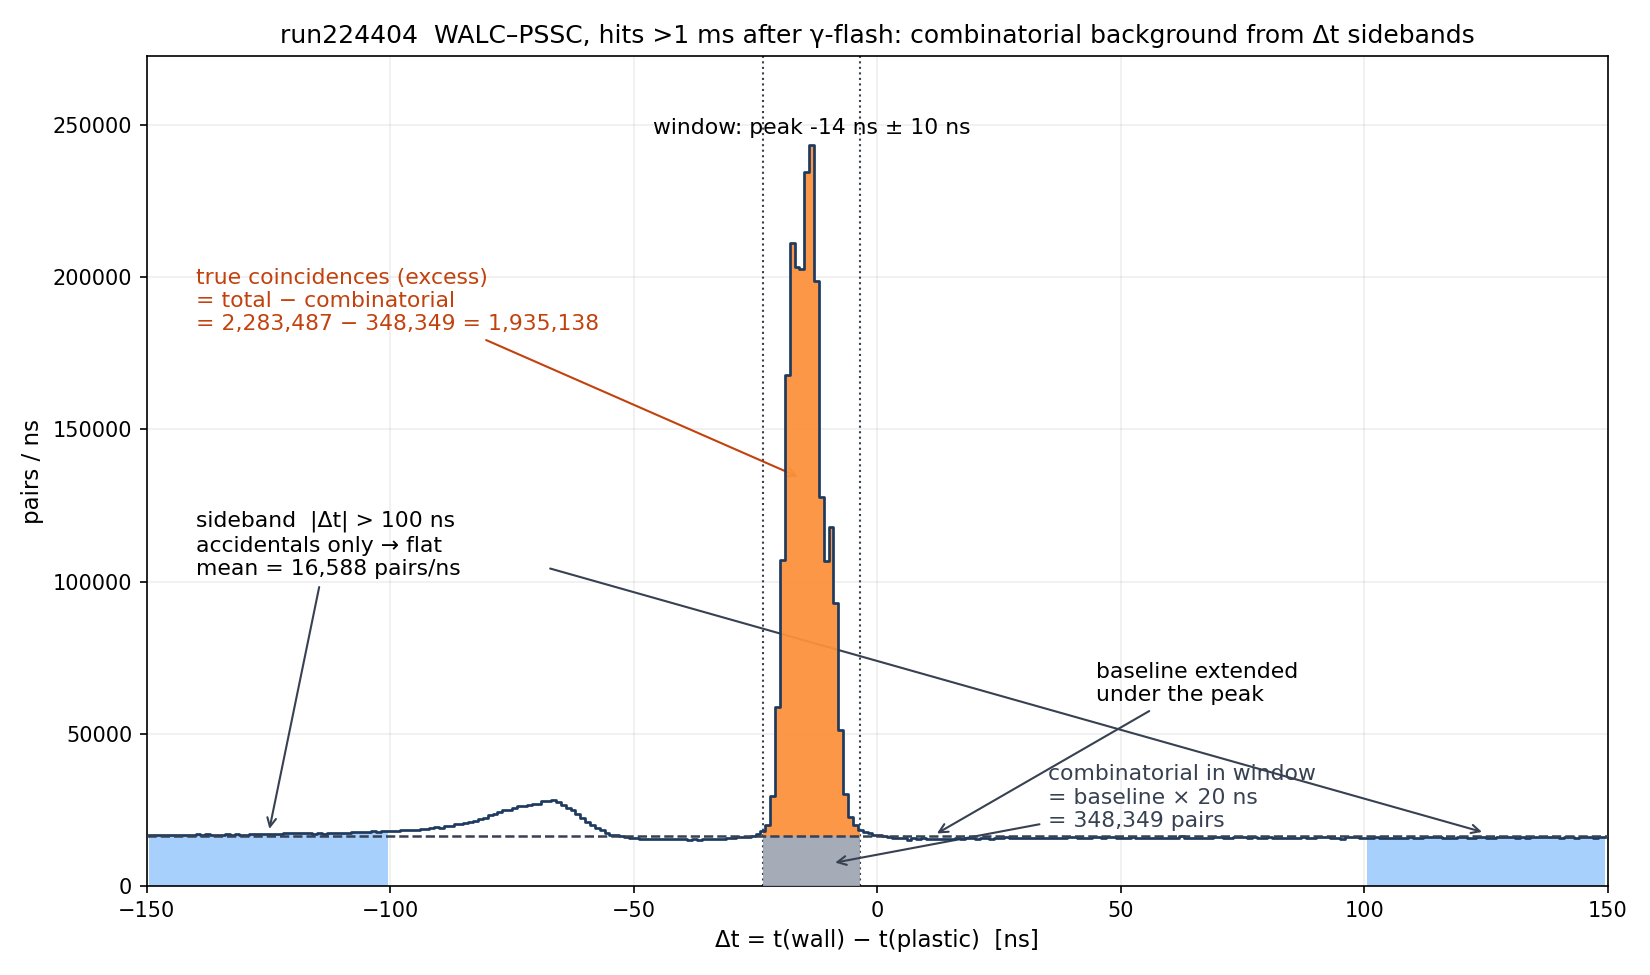
\includegraphics[width=.75\textwidth]{05_sideband_diagram/sideband_method.png}
\caption{Combinatorial-background estimation on real data (WALC--PSSC,
$>$\SI{1}{\milli\second} after flash).}
\label{fig:sideband}
\end{figure}

\section{Detector mapping confirmed in data}
Within each wall, the channel--channel coincidence matrix is block-diagonal in
the pairs (1,2),(3,4),(5,6),(7,8): each pair is the top/bottom readout of one
4-bar group (2.2--2.6M excess pairs each, 52--91\% of a channel's
coincidences; top--bottom $\Delta t$ rms $\sim$2.5\,ns). Groups are ordered
left$\to$right (seen from the back) across the two plastic bars. Which slot is
top remains \emph{assumed} (odd = top) pending the cabling sheet. Cross-arm
matrices show corner hotspots --- WALA(7,8)$\times$WALD(1,2) and
WALB(1,2)$\times$WALC(7,8) --- identifying A--D and B--C as \emph{adjacent}
arms (ring order consistent with A$\to$D$\to$C$\to$B).

\begin{figure}[H]\centering
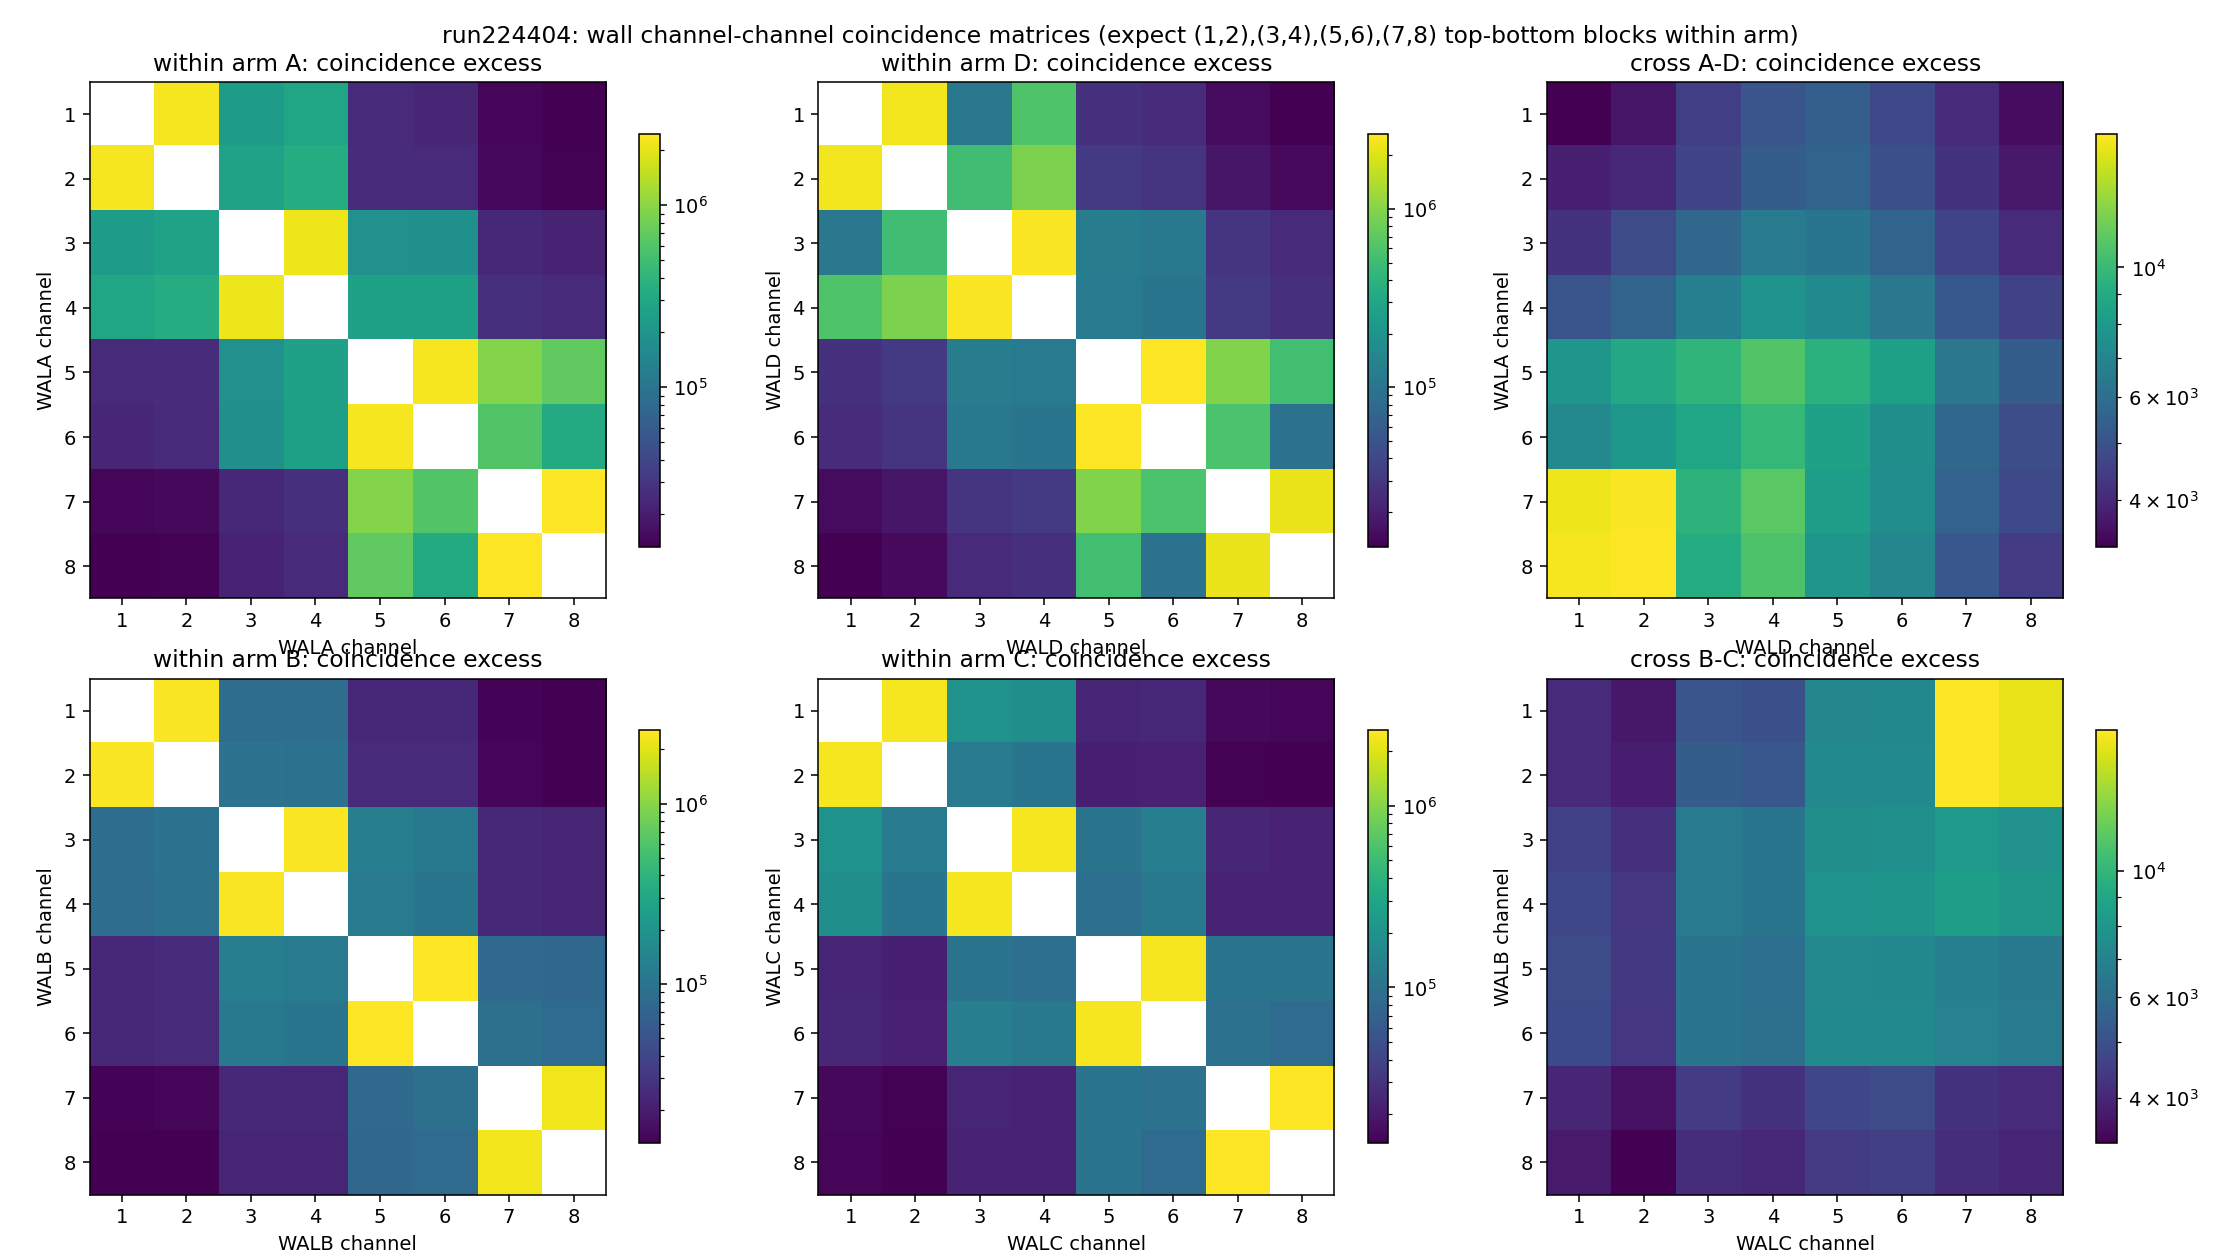
\includegraphics[width=.9\textwidth]{06_07_geometry_mip/wall_geometry_matrices.png}
\caption{Wall channel--channel coincidence matrices: within-arm top/bottom
blocks (left, middle) and cross-arm corner hotspots (right).}
\end{figure}

\section{SiPM-wall MIP calibration (arms B, C)}
The sideband-subtracted coincidence amplitude spectra of WALB/WALC show clean
Landau-like MIP peaks in all 16 channels, well separated from threshold
(Fig.~\ref{fig:mip}). Peaks span \SIrange{29.4}{38.9}{\milli\volt}
($\sim$25\% channel-to-channel spread), giving direct per-channel MIP
calibration constants. Note the physics of the selection: the plastic sits at
the \emph{back} of the arm, so the coincidence requires the track to traverse
the wall and reach the plastic --- a genuine through-going (MIP) selection for
the \emph{wall}. For the \emph{plastic} itself the same selection only
requires a hit, so the plastic spectra are hit spectra (including
stopping/soft particles), not MIP spectra.

\begin{figure}[H]\centering
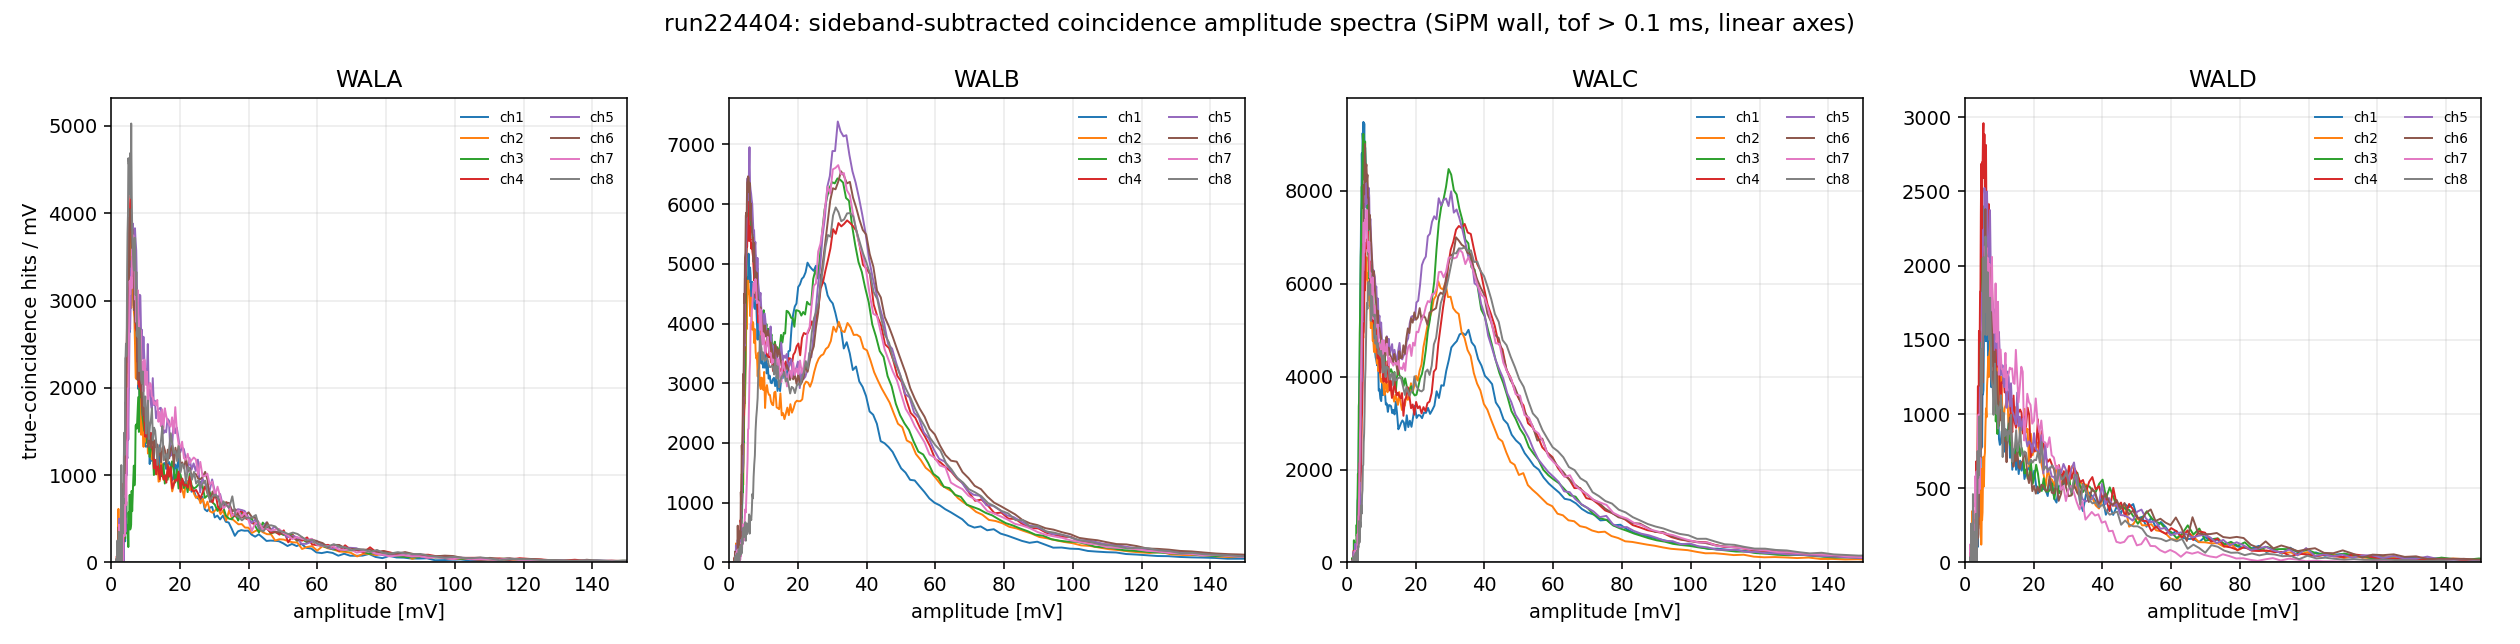
\includegraphics[width=\textwidth]{06_07_geometry_mip/mip_wall_spectra_linear.png}
\caption{Sideband-subtracted wall coincidence amplitude spectra (linear, mV).
B and C: clean MIP peaks; A and D: no MIP population.}
\label{fig:mip}
\end{figure}

\begin{figure}[H]\centering
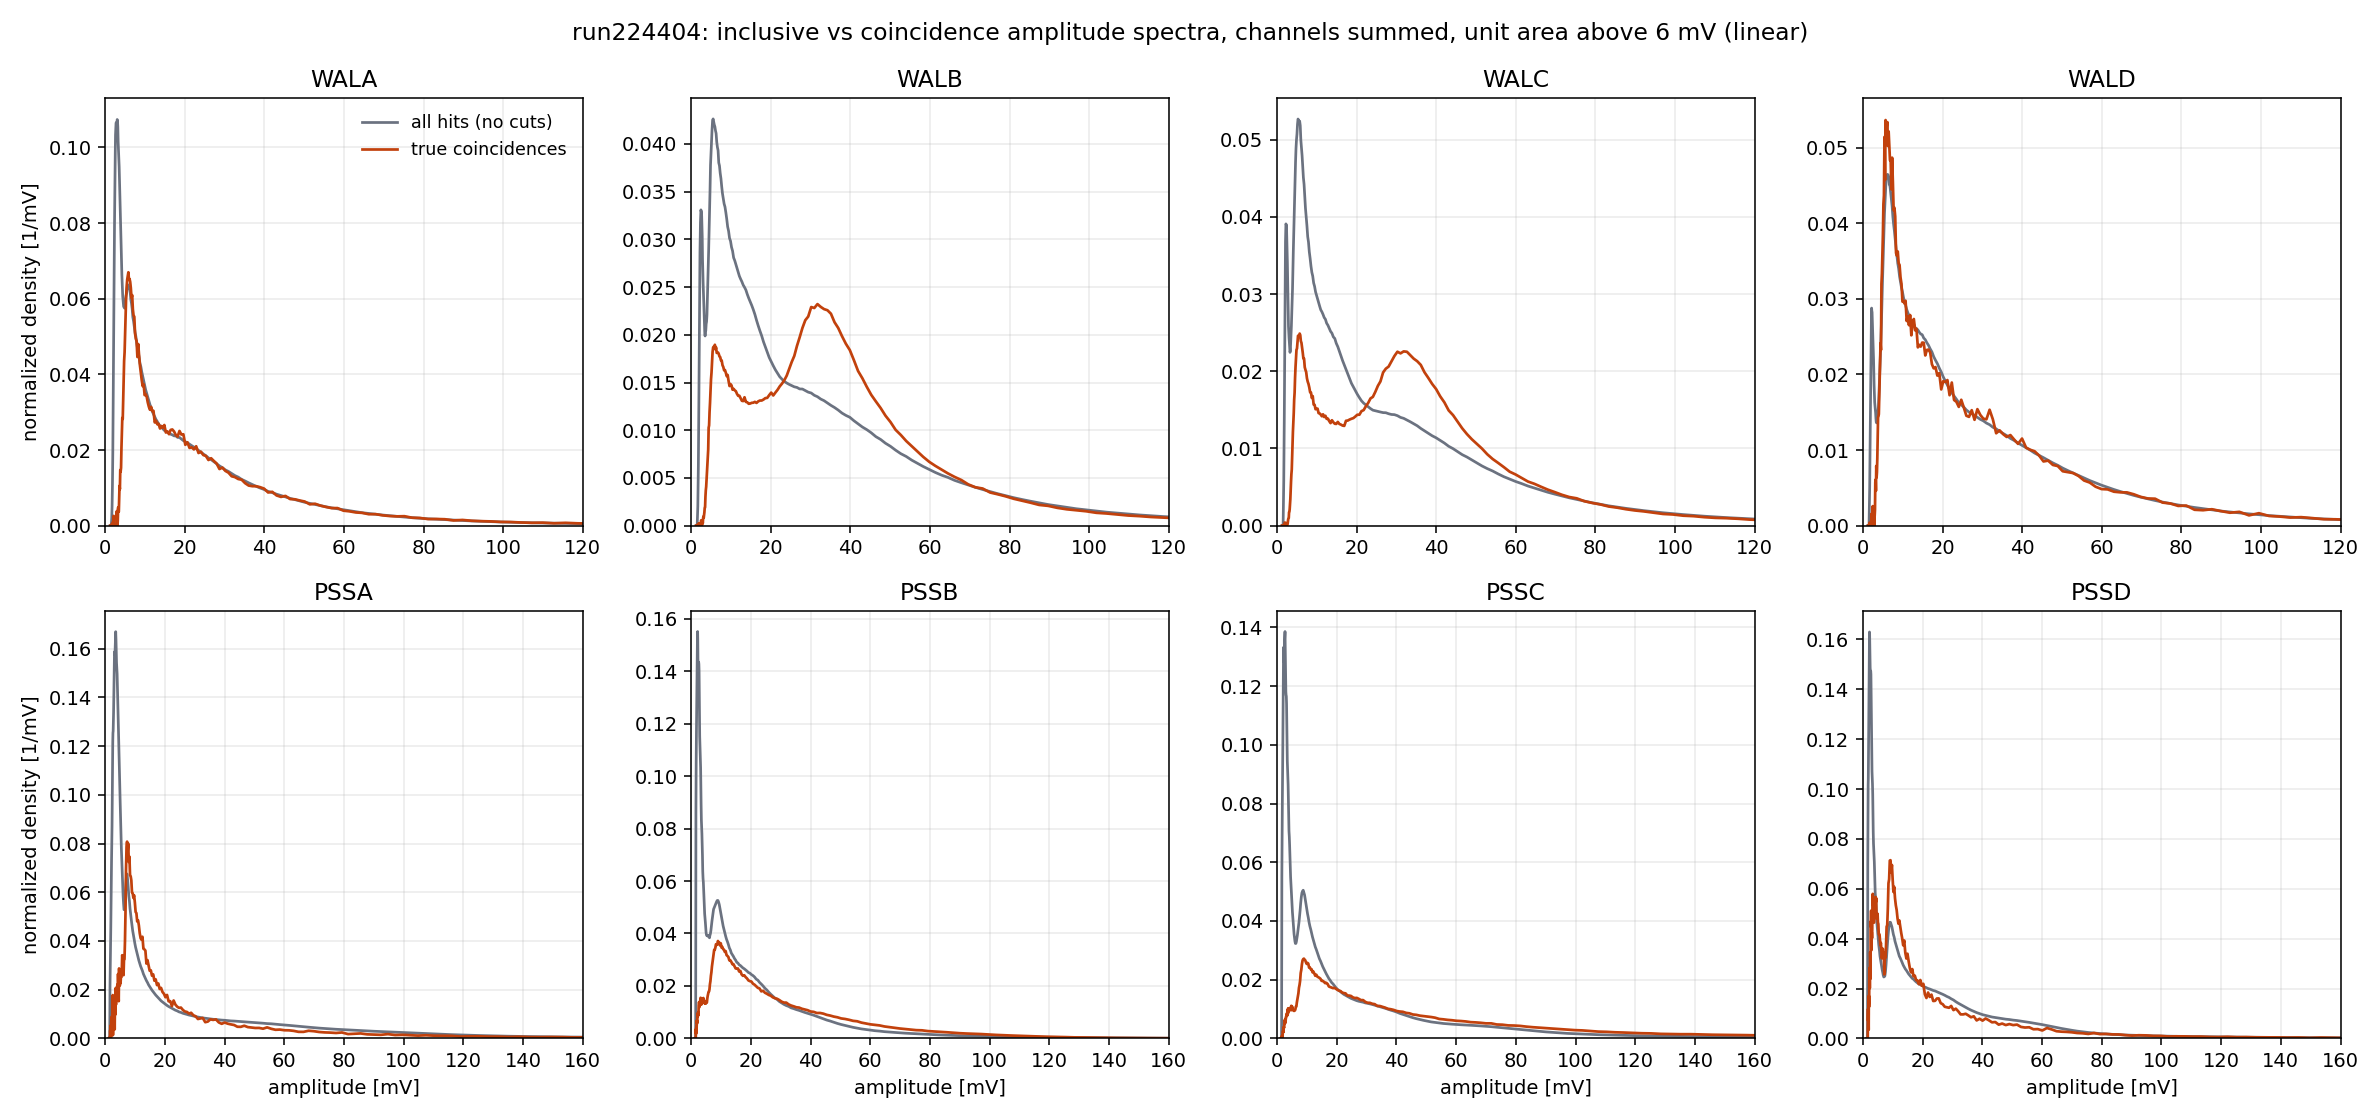
\includegraphics[width=\textwidth]{08_inclusive_vs_coinc/inclusive_vs_coinc_linear.png}
\caption{Inclusive vs coincidence-selected spectra (unit area): the
coincidence isolates the MIP bump on B/C; on A/D it merely traces the
inclusive shape.}
\end{figure}

\section{The A/D problem}
Arms A and D produce 6--8$\times$ fewer true coincidences than B/C and their
coincident wall spectra show \emph{no} MIP bump --- above $\sim$15\,mV they
simply trace the inclusive shape. Hypotheses: (i) plastic PMT gain/threshold
too low on A/D, so MIP tracks fail to fire the plastic; (ii) wall SiPM gain
low; (iii) geometry/orientation: A/D simply see less through-going flux.
Inclusive plastic medians are within $\pm$30\% across all eight PMTs (PSSD1
highest), disfavoring a large plastic-gain deficit.

A wall-only cross-check --- coincidences between the top and bottom SiPMs of
the same 4-bar group (Fig.~\ref{fig:topbot}) --- shows a MIP-scale bump at
25--40\,mV on all four arms, so the SiPM response and gain are healthy
everywhere, and every wall channel has an amplitude landmark. This check is
\emph{not} conclusive about the cause of the A/D deficit, however: top and
bottom view the same scintillator, so a single localized deposit --- including
a $\gamma$ Compton-scattering in the bars --- lights both ends in tight
coincidence. It therefore removes electronics noise but cannot distinguish
through-going tracks from local deposits, and says nothing about whether
particles continue to the back plastic. The A/D deficit remains
unattributed among: plastic response, absorption between wall and plastic
(e.g.\ if A/D carry the liquid-scintillator layers in front of the plastic ---
consistent with LIQA/LIQD being the cabled liquid channels, but unconfirmed),
or a softer/more $\gamma$-rich flux at those arms. Discriminating follow-ups:
the pre-flash cosmic sample (guaranteed through-going muons --- do A/D
wall--plastic coincidences appear at the expected rate?), the LIQ readout, and
a plastic HV scan.

\begin{figure}[H]\centering
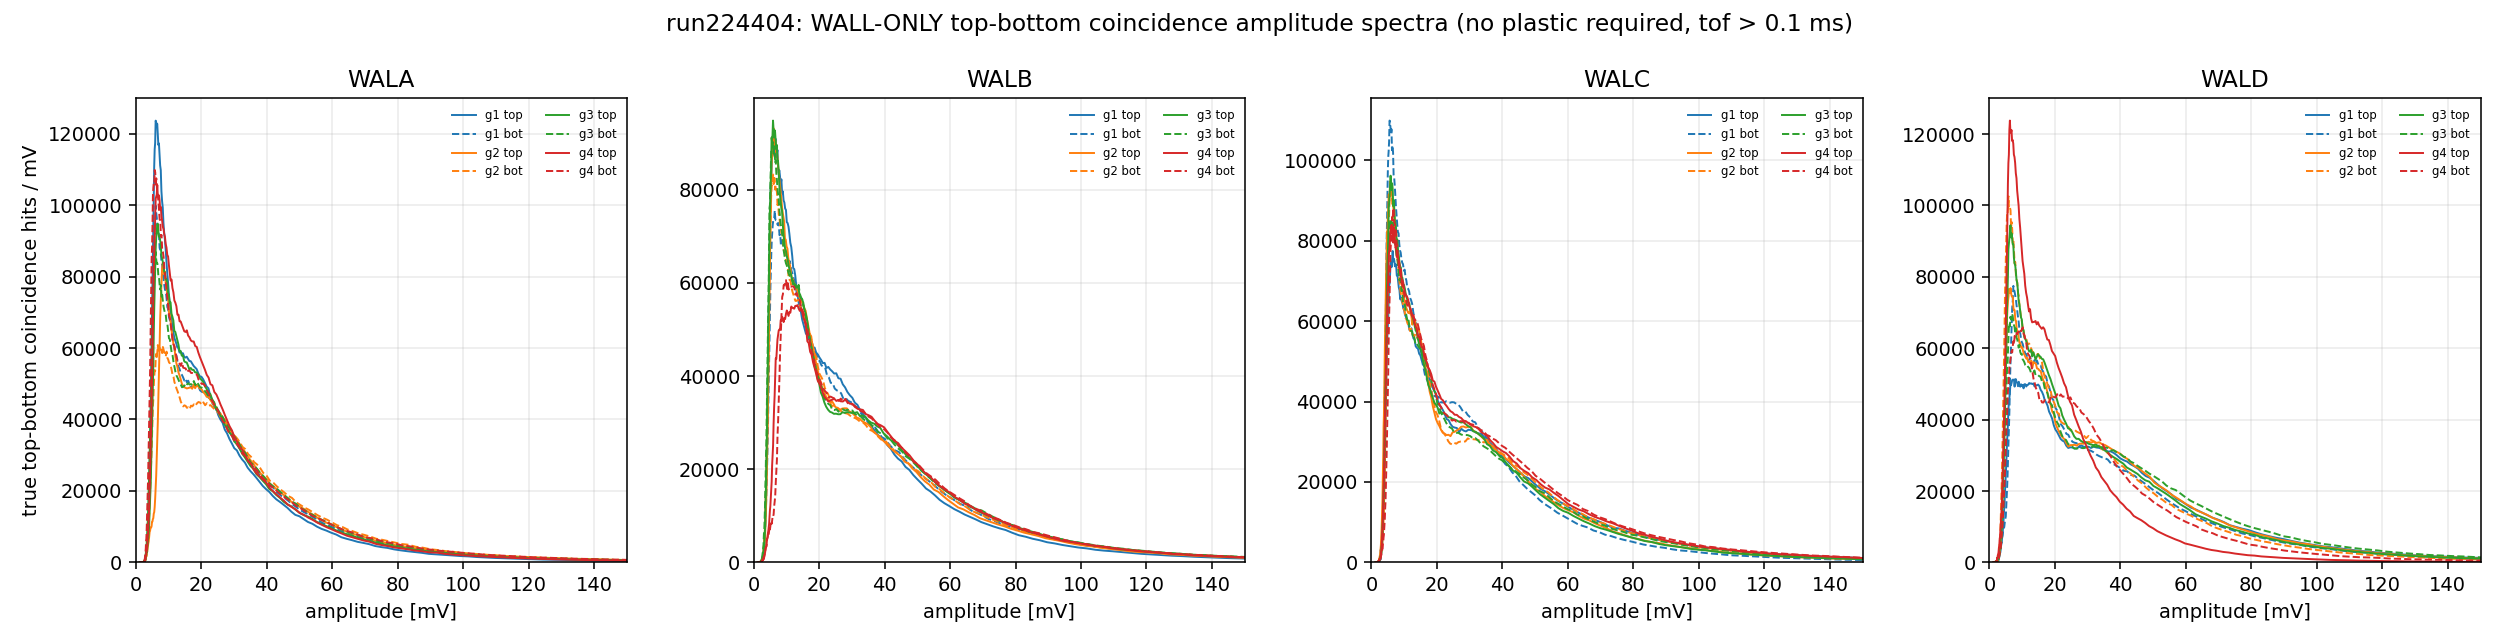
\includegraphics[width=\textwidth]{06_07_geometry_mip/wall_topbot_spectra.png}
\caption{Wall-only top--bottom coincidence amplitude spectra (sideband
subtracted): MIP-scale bump on all arms. Note top/bottom read the same bars,
so this selects any real deposit, not through-going tracks.}
\label{fig:topbot}
\end{figure}

\section{Plastic PMT gains and HV suggestions}
Relative gains from inclusive spectral medians (cross-arm comparable) with
$G\propto V^{7}$:

\begin{table}[H]\centering\small
\begin{tabular}{lrrrrr}
\toprule
PMT & HV [V] & median$_\mathrm{inc}$ [mV] & rel.\ gain & $V$ (equalize) & $V$ ($2\times$) \\
\midrule
PSSA1 (AL) & 1325 & 10.4 & 0.74 & 1384 & 1528 \\
PSSA2 (AR) & 1275 & 13.2 & 0.93 & 1288 & 1422 \\
PSSB1 (BL) & 1325 & 13.1 & 0.93 & 1339 & 1478 \\
PSSB2 (BR) & 1300 & 14.9 & 1.05 & 1290 & 1425 \\
PSSC1 (CL) & 1300 & 14.5 & 1.03 & 1295 & 1429 \\
PSSC2 (CR) & 1300 & 15.3 & 1.08 & 1285 & 1419 \\
PSSD1 (DL) & 1300 & 17.8 & 1.26 & 1258 & 1389 \\
PSSD2 (DR) & 1300 & 14.9 & 1.06 & 1290 & 1424 \\
\bottomrule
\end{tabular}
\caption{Plastic PMT relative gains and HV suggestions ($\alpha=7$ assumed;
calibrate with a 2-point HV scan before trusting shifts $>$25\,V).}
\end{table}

\section{Requests}
\begin{enumerate}
\item \textbf{Read out the liquid scintillators} (LIQ; behind the plastic).
A wall+LIQ coincidence requires passage \emph{through} the plastic, isolating
MIPs in the plastic and giving its true MIP calibration. Only LIQA/LIQD are
cabled and neither is writing data.
\item Plastic HV scan (2 points suffice) to calibrate gain vs voltage, then
apply the equalization above.
\item Confirm from cabling: top vs bottom SiPM card assignment; which 4 of the
20 wall bars are unread; physical positions of arms A--D.
\item Investigate the SiPM-wall outage (bunches 643--2212) with the DAQ crew.
\end{enumerate}

\end{document}
